%%%%%%%%%%%%%%%%%%%%%%%%%%%%%%%%%%%%%%%%%%%%%%%%%%%%%%%%%%%%%%
% NUbots' TDP 2016
%
% Date: 08.02.2016
%
%
\documentclass{llncs}
%
\usepackage{graphicx}
%
\begin{document}
%

\frontmatter          % for the preliminaries
%
\pagestyle{headings}  % switches on printing of running heads
\addtocmark{The NUbots Qualification material for RoboCup 2016} % additional mark in the TOC
%
%
\mainmatter              % start of the contributions
%
\title{The NUbots Team Description Paper 2016}
%
\titlerunning{The NUbots Team Description for 2016}  % abbreviated title (for running head)
%                                     also used for the TOC unless
%                                     \toctitle is used

\author{Trent Houliston
		\and Jake Fountain
		\and Anita Sugo
        \and Mitchell Metcalfe
		\and Alexandre Mendes
        \and Peter Turner
        \and Elliot Catt
        \and Tony Jackson
        \and Zachary Mason-Roach
        \and Alex Biddulph
        \and Stephan K. Chalup
        }
%
\authorrunning{Houliston et al.}   % abbreviated author list (for running head)
%
%%%% modified list of authors for the TOC (add the affiliations)
\tocauthor{
T. Houliston,
J. Fountain,
A. Sugo,
M. Metcalfe,
A. Mendes,
P. Turner,
A. Biddulph,
S.K. Chalup}

%
\institute{Newcastle Robotics Laboratory\\ School of Electrical Engineering \& Computer Science\\
Faculty of Engineering and Built Environment\\
The University of Newcastle, Callaghan 2308, Australia\\
Contact: \email{stephan.chalup@newcastle.edu.au}\\
Homepage: \texttt{http://robots.newcastle.edu.au}}
%

\maketitle              % typeset the title of the contribution

\begin{abstract}
In 2016 the NUbots team will represent The University of Newcastle, Australia, in the RoboCup Kidsize Humanoid League. The NUbots have participated in RoboCup since 2002. They won the title in the RoboCup Four Legged League in 2006 and as part of the NUManoids team they won the title in the Standard Platform League in 2008. The team's main research addresses interdisciplinary applications of machine learning, software engineering and computer vision. This paper summarizes the history of the NUbot team and describes the roles and research interests its team members. The paper also gives an overview of the NUbots'  software system and the NUbots' main platform, the Darwin-OP with minor modifications.

%The NUbots team, from The University of Newcastle, Australia, has had a strong record of success in the RoboCup Standard Platform League since first entering in 2002. The team has also competed within the RoboCup Humanoid Kid-Size League since 2012. The 2014 team brings a renewed focus on software architecture, modularity, and the ability to easily share code. This paper summarizes the history of the NUbots team, describes the roles and research of the team members, gives an overview of the NUbots' robots and software system, and addresses relevant research projects within the the Newcastle Robotics Laboratory.
\end{abstract}

%
\section{Introduction}
The NUbot robot soccer team has been the central project of the Newcastle Robotics Laboratory since 2002. The goal of the NUbot team is to demonstrate exiting state-of-the-art team play in the RoboCup Kidsize Humanoid League and ultimately win the competition.

Several research projects at undergraduate and postgraduate levels are associated with the NUbot team. Most projects are associated with the necessary tasks required to make the team play well in the competition. Additional areas of special research interest include machine learning on robots \cite{ChalupEtAlSMC2007,FountainEtAl2014}, computer vision \cite{MetcalfeEtAl2016}, software engieering for robots \cite{HoulistonEtAlNUClear2016} and combinations with virtual reality~\cite{FountainChalup2015}.

The Nubots' mission is to contribute to a responsible development and application of robotics and to develop and program robots that can support humans not only for routine, challenging, or dangerous tasks, but also to improve quality of life through personal assistance, companionship and coaching. Some of our projects therefore emphasise anthropocentric and biocybernetic aspects in robotics including research on robot emotions~\cite{ChalupOstwald2009,WalkerChalup2015,HongEtAl2014,WongEtAl2012,WongEtAl2013}.


%The central goal of the NUbots is to be a high performance competitive robot soccer team at RoboCup. The vision of the research projects associated with the NUbots team is to develop and program robots that can support humans not only for routine, challenging, or dangerous tasks, but also to improve quality of life through personal assistance, companionship, and coaching.   This includes new aspects of human robot interaction and perception. The Newcastle Robotics Laboratory hosts several postgraduate and undergraduate research projects that are associated with the NUbots.

%The following sections describe the history of the team, the roles and research of the team members and addresses associated research projects and relevant aspects of the study and research environment of the University of Newcastle, Australia.

\section{Commitment to RoboCup 2016}
The NUbots commit to participation at RoboCup 2016 upon successful qualification. We also commit to provision of a person, with sufficient knowledge of the rules, available as referee during the competition.

\section{History of the NUbots' participation at RoboCup}
%The University of Newcastle's RoboCup initiative started in 2001. After the introduction of new robotics and machine learning
%related courses and projects two undergraduate students participated in RoboCup Junior in Seattle and won the world title.
The NUbots team, from the University of Newcastle, Australia, competed in the Four-Legged-League from 2002-2007 using Sony AIBO ERS-210 and ERS-7 robots. The NUbots participated for the first time at RoboCup 2002 in Fukuoka in the Sony Four-Legged League (3rd place). At RoboCup 2006 in Bremen, Germany, the NUbots won the title. %Scenes from the final game are available at

From 2008 to 20011 they used the Aldebaran Nao within the Standard Platform League. They achieved a first place in 2008 as part of the NUManoid team in Suzhou, China.

The NUbots joined the Kidsize Humanoid League in 2012 with the DARwIn-OP robots, and ported their SPL codebase to the new platform. The NUbots retained a robust and fast vision and localisation system from the SPL, and ported the B-human NAO walk to the DARwIn-OP for 2012-2013. In 2015 the NUbot team reached the quarter finals. They used small modifications of the head and feet and a complete rewrite of their software system based on their new NUClear operating system.

%During the previous two years the NUbots SPL code base has been ported to the DARwIn-OP platform and the majority of modules previously used on the NAO robot in the SPL were fielded for RoboCup 2012. Since then the majority of modules have undergone major revision in order to allow more effective use of the newer platform and in response to recent changes in the league rules.

\section{Background of the NUbots Team Members}

\begin{itemize}
\item \emph{Trent Houliston} is studying for a Doctorate of Philosophy in Software Engineering and is the NUbots team leader. His research topic is Software Architecture for Robotics and Artificial Intelligence. He designed and implemented the new architecture for the robots, and aided in the development of many of the components.

\item \emph{Jake Fountain} is studying for a Doctorate of Philosophy in Computer Science and is the Team Manager. Jake has undergraduate degrees in mathematics and science, majoring in physics, with Honours in Computer Science~\cite{FountainChalup2015}. His main interests lie in virtual reality and robotics.

\item \emph{Anita Sugo} is a fourth year undergraduate student studying a degrees in mathematics and science, with a major in physics. She is interested in the mathematics used in robotics and is currently working on computer vision.

\item \emph{Mitchell Metcalfe} has undergraduate degrees in mathematics and computer science, with Honours in Computer Science. He contributes to the NUbots' localisation, and motion planning systems, and has interests in computer vision and machine learning.

\item \emph{Elliot Catt} is a final year undergraduate student studying a Bachelor of mathematics degree. His interests include number theory,  machine learning and intelligent agents \cite{CattCoonsVelich}. He is currently working on a sound based localisation project and behaviour.

\item \emph{Matthew Amos} is a third year undergraduate student studying a combined degree in Computer Science and Computer Engineering. He is interested in computer vision and machine learning.

\item \emph{Tony Jackson} is a fifth year undergraduate student studying a combined degree in Computer Science and Computer Engineering. He has recently joined the NUbots team and has been contributing towards the walk engine of the robot.

\item \emph{Zachary Mason-Roach} is a final year undergraduate student studying a combined Bachelor degree in Computer Science and Computer Engineering (Honours). He is presently contributing to the NUbots walk engine and designing balance and push-recovery methods for humanoid robotics.  His dominant interests comprise of machine learning and robotic awareness, computer vision and mathematical applications to artificial intelligence.

\item \emph{Luke Farrawell} is a third year undergraduate student studying Software Engineering (Honours). His interests include robotics and computer graphics. He contributes to NUsight; the real-time web based debugging environment.

%\item \emph{Steven}

\item \emph{Alex Biddulph} is completing the final semester of his undergraduate degree in Computer Engineering and Computer Science. He will then be commencing his Doctorate of Philosphy in Computer Engineering where he will be studying the symbiotic relaitonship between hardware and algorithms, with a focus on computer vision.

\item \emph{Peter Turner} is technical staff in the School of Electrical Engineering and Computer Science. Peter provides hardware support and assists the team with physical robot design upgrades. %an expert on robot hardware and electronics and familiar with the DARwIn-OP.

\item \emph{Dr. Alexandre Mendes} is deputy head of the Newcastle Robotics Lab. He is a Senior Lecturer in Computer Science and Software Engineering. He joined the group in September 2011 and his research areas are algorithms and optimisation.

\item \emph{Associate Professor Stephan Chalup} is the head of the Newcastle Robotics Lab and of the Interdisciplinary Machine Learning Research Group (IMLRG). He is one of the initiators of the University of Newcastle's RoboCup activities since 2001. His research interests include machine learning, pattern recognition and anthropocentric robotics.

\end{itemize}
We also acknowledge the valuable input of colleagues from the Newcastle Robotics Laboratory, team members of previous years
and the Interdisciplinary Machine Learning Research Group (IMLRG) in
Newcastle, Australia. Details are linked to the relevant webpages at
\texttt{www.robots.newcastle.edu.au}.

%\pagebreak
\section{Software and Hardware Overview}
The NUbots team's software source is available from \cite{nubotsGit} and is covered under the GPL. This code includes associated toolkits for building and deploying the software. Our software is designed to work on multiple robotic platforms, and all of the individual modules have been designed to be easily used in other systems. The flexibility of our approach has been demonstrated in a deployment of the NUbots vision system on a marine platform and is currently also ported to a larger humanoid platform.% \cite{renton2014robotx}. % The sensors and actuators are accessed using a standard format, regardless of the robot running the software~\cite{Kulk2011c}.

Following development of a new software system in 2014 and 2015, the NUbots are now focusing on current and emerging challenges within the RoboCup Kid-size League. These include robust, adaptable image segmentation; generic ball detection; and improving the architecture of current walk engines to cope with the new artificial grass surface. The NUbots software is designed to allow new teams and team members to easily understand and innovate on existing code, and is made freely available to encourage research and innovation.

%This year marks a major change in the software architecture of the NUbots, with improved software modularity coming from a cutting edge event based message passing system. The NUbots' architecture now has strong parallels with ROS (although without the associated overheads) and interoperability with ROS modules is planned. The NUbots software is designed to allow new teams and team members to easily understand and innovate on existing code. We plan to provide a full code release post RoboCup 2014.

%The software is broken into a number of modules. The primary modules are: vision, localisation, behaviour, and motion. An overview of our software structure can be seen in Figure~\ref{fig:platform}. The research areas applied to each of these modules are described in the research section.

%\begin{figure}[bht!]
%\begin{center}
%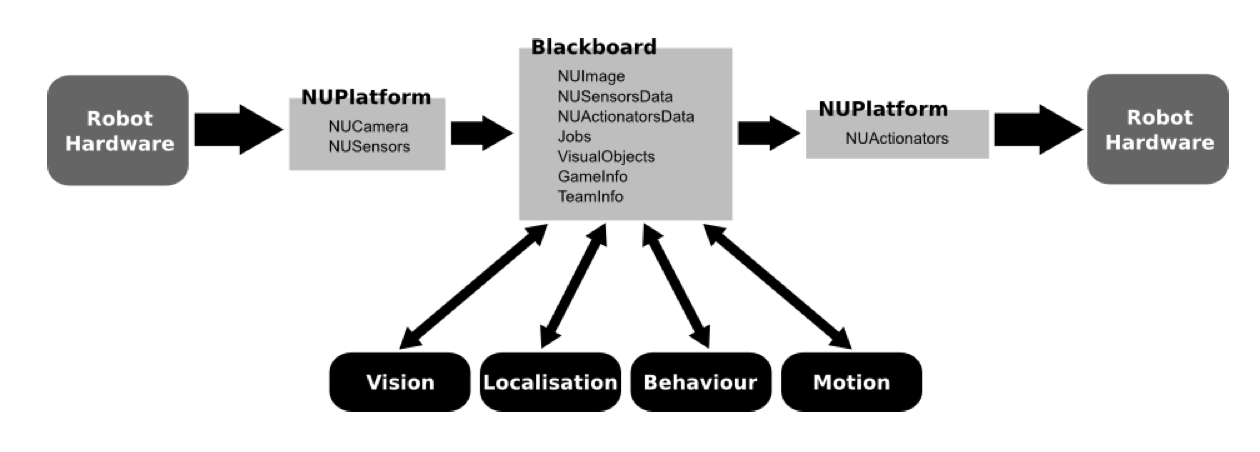
\includegraphics[width=1.0\textwidth]{Platform.png}
%\caption{An overview of the software framework, and the transfer of information between the hardware and software modules via the blackboard~\cite{Kulk2011c}.}
%\label{fig:platform}
%\end{center}
%\end{figure}

The NUbots use seven DARwIn-OP robots with small modifications such as foot sensors and a new head.
%The team has seven of these robots that are of the standard design with the exception of a slightly reduced foot size. %The team also hopes to field modified DARwIn-OP robots consisting of a full HD camera, an ODroid-XU computer and an updated motor communications board as a part of a student project. %Aditional minor structural modifications as well as a replacement of the main processor are planned after RoboCup 2013.

%\begin{figure}
%\begin{center}
%\scalebox{0.26}{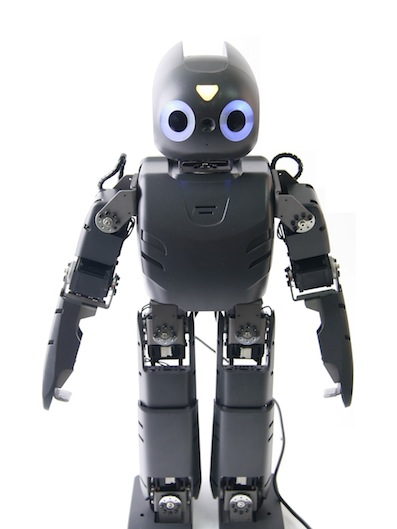
\includegraphics{darwin.png}}
%\caption{The DARWIN-OP Robot.}
%\label{fig:darwin}
%\end{center}
%\end{figure}

\subsection{Hardware Enhancements since RoboCup 2014/2015}
At RoboCup 2014 we trialed rapid prototyping for a new head design for the Darwin-OP robots to fit upgraded Logitech C920 cameras. %Since this time we have been improving designs and readying for an open source release once remaining issues are resolved. We field these otherwise standard Darwin-OP robots under the name NU-Darwin.

We have been partnering with Kontron Australia to develop more powerful embedded pc boards in order to upgrade our capabilities and deploy new robotics platforms. This upgrade will see higher quality accelerometers and gyroscopes and more hardware communications channels added to the robots, as well as an upgrade to a quad-core celeron platform with access to OpenCL.

At the 2015 competition soccer studds were added to the feet to allow a more stable walk.

For 2016 it is planned to integrate a taller robot based on the Igus/Nimbro platform family into the NUbot team.
%Since RoboCup 2013, improvements have been made in the area of software architecture and hardware. As the league moves to more realistic game conditions, we are trialling a hardware control platform composed of the following:

%In response to the increase in field size, the Logitech C905 is being replaced with a Logitech C920. The new camera will provide a 1080p image, allowing the robots to detect and classify objects at greater distances.

%The Main Controller (CompuLab fit-PC2i) is being replaced by an ODroid-XU to provide the extra processing power that is required for processing the images from the Logitech C920.

%A prototype hardware replacement for the ROBOTIS CM730 Sub Controller, named the TAJ3850, is
%being developed as part of a Computer Engineering Third Year Project. The TAJ3850 provides power to all system components, a battery monitoring system featuring a low-voltage alarm and an extremely low-voltage automatic cut-off, an improved six-axis motion processing unit, a temperature sensor, and five dedicated motor buses. The TAJ3850 also exposes peripheral connections from the ODroid-XU to the back panel of the robot (HDMI, USB3, LAN, Audio output), monitors the three back-panel control buttons, and controls the status LEDs on the back panel and in the head.

%\begin{figure}
%\begin{center}
%\scalebox{0.3}{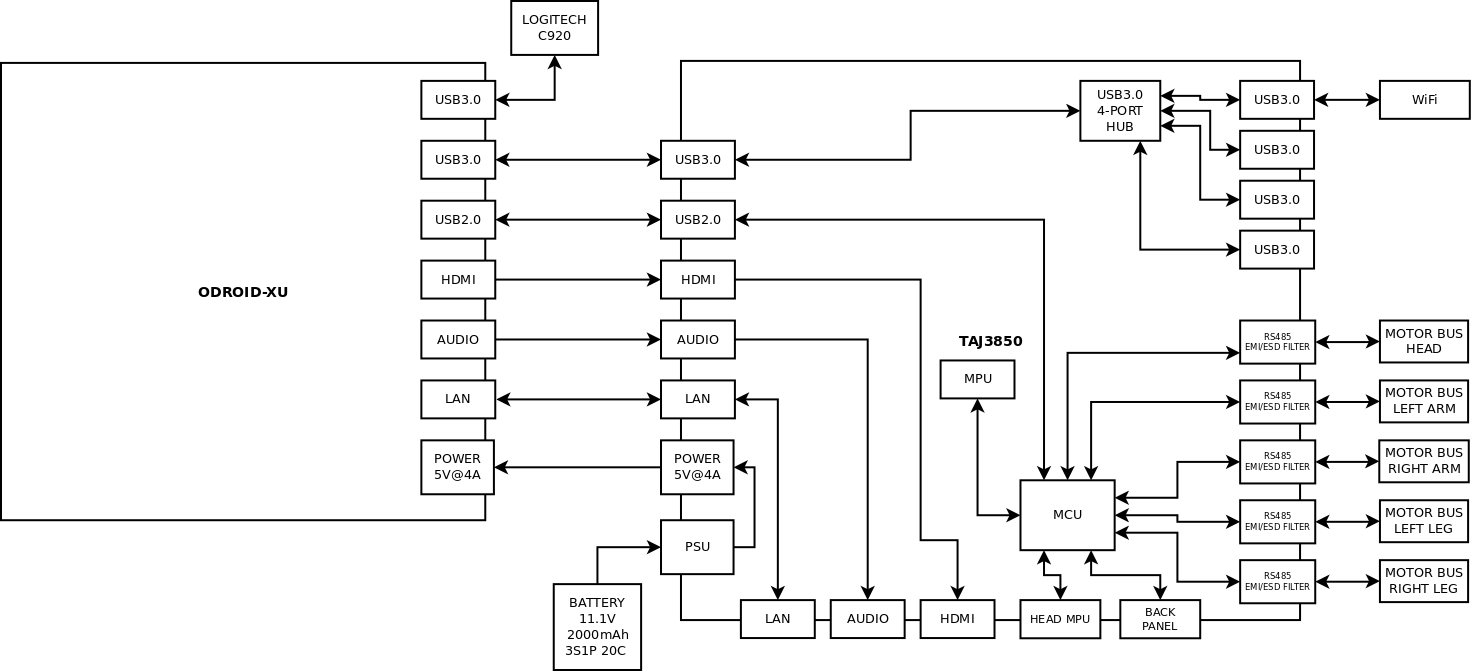
\includegraphics[angle=270]{TAJ3850.png}}
%\caption{Connection mappings between the TAJ3850, ODroid-XU, and external peripherals.}
%\label{fig:taj3850}
%\end{center}
%\end{figure}

%The above enhancements will not be implemented on all of the DARwIn-OP robots.
\subsection{Acknowledgement of Use of Code}
The NUbots DARwIn-OP robots use a walk engine based on the 2013 Team Darwin code release. We acknowledge the source of this code. The NUbots have ported this code to C++ and restructured the logic, making numerous structural and technical changes since. %The source for this module can be found in \cite{nubotsGit2}.

\section{Research Areas}

\noindent\textbf{Robot Vision:} Vision is one of the major research areas associated with the Newcastle Robotics Laboratory. Several subtopics have been investigated including object recognition, horizon determination, edge detection, model fitting and colour classification using ellipse fitting, convex optimisation and kernel machines. Recent work has resulted in a fully-autonomous method of colour look-up table adaptation for changing lighting conditions, allowing us to overcome one of the major limitations of the colour look-up table system. Publications are available e.g. from~\cite{budden2012colour,budden2012ball,henderson_2007,nicklin_2007,NUBOT2006,Henderson2008,flannery2013ransac,budden2013salient,HoulistonEtAl2015,MetcalfeEtAl2016}.

%\noindent\textbf{Localisation and Kalman Filters:} Research on the topic of localisation focused on Bayesian approaches to robot localisation including Kalman Filter and particle filter based methods. We are interested in modifications of the Kalman Filter to handle non-ideal information from vision, incorporate increased information from multiple agents, and effectively utilise non-unique objects.
%Furthermore we are also interested in the use of machine learning to
%improve the models used by localisation. For information about our current approach see
%\cite{robocup_2009}.

\noindent\textbf{Development of the Robot Bear:} In a collaborative effort with the company Tribotix and colleagues in design, a bear-like robot (called Hykim) was developed~\cite{ChalupEtAl2006}. It has a modular open platform using Dynamixel servos.

\noindent\textbf{Biped Robot Locomotion:} The improvement of walking speed and stability has been investigated by the NUbots for several years and on different platforms: On the AIBO robot we achieved one of the fastest walks at that time by walk parameter evolution \cite{QuinlanEtAlACRA2003,ChalupEtAlSMC2007}. On the Nao robot we improved existing walk engines by modifying the joint stiffnesses, or controller gains, \cite{Kulk2008,Kulk2010} and by applyinmg optimisation. % Kulk2010a
%The stiffnesses were selected through an iterative process to maximise the cost of transport. We investigated the application of Support Vector Machines and Neural Networks to proprioception data for sensing perturbations during pseudo quiet stance. Walk improvements have been primarily done via optimisation techniques \cite{Kulk2011a},  %,Kulk2011b
%with recent improvements to our framework for online optimisation of bipedal humanoid locomotion.
The use of spiking neural networks has been trialled in simulation~\cite{WiklendtChalup2008}. Prior to RoboCup 2012 the walk engine developed by the leading SPL team BHuman~\cite{BHumanWalk2010} was ported to the DARwIn-OP platform, and a variety of optimisation techniques were developed and successfully applied to improve walking speed and stability of the DARwIn-OP walk. %\cite{budden2013probabilistic}. Multi-agent walk optimisation is being developed for this year's competition.

\noindent\textbf{Reinforcement Learning, Affective Computing and Robot Emotions:} We investigate the feasibility of reinforcement learning or neurodynamic programming for applications such as motor control and music composition. Concepts for affective computing are developed in multidisciplinary projects in collaboration with the areas of architecture and cognitive science. The concept of emotion is important for selective memory formation and action weighting and continues to gain importance in the robotics community, including within robotic soccer~\cite{HongEtAl2014,FountainEtAl2014,ChalupOstwald2009,WalkerChalup2015,WongEtAl2012,WongEtAl2013}.

\noindent\textbf{Gaze analysis and head movement behavioural learning:} We investigated methods for human and robot pedestrian gaze analysis in~\cite{JalalianEtAl_CAADRIA2011,WongEtAl2012} as well as space perception, way finding and the detection and analysis of salient regions~\cite{BhatiaEtAl2013,BhatiaChalupOstwald2013}. Recently we applied motivated reinforcement learning techniques to optimising head movement behaviour, providing a robust algorithm by which a robot learns to choose landmarks to localise efficiently during a soccer game~\cite{FountainEtAl2014}.

\noindent\textbf{Manifold Learning:} In several projects we
investigate the application of non-linear dimensionality reduction
methods in order to achieve more understanding of, and more precise
and efficient processing of, high-dimensional visual and acoustic data \cite{ChalupEtAl2007b,WongEtAl2012,WongChalup2008}

\noindent\textbf{Software Engineering for Robotics:} Much work has been focused on the underlying software architecture and external utilities to enable flexibility and extensibility for future research \cite{Kulk2011c,HoulistonEtAlNUClear2016}. Projects undertaken include improving the configurability of the software system via real-time configuration updates, development of a web-based online visualisation and debugging utility \cite{AnnableEtAl2014} and the application of software architectural principles to create a multithreaded event-based system with almost no run-time overhead. Some of this work is still in progress by new undergraduate and postgraduate students who are associated with the lab \cite{BilleEtAl2016}.

\section{Related Research Concentrations}
The \emph{Interdisciplinary Machine Learning Research Group (IMLRG)} investigates different aspects of machine learning and data mining in theory, experiments and applications. The IMLRG's research areas include: Dimensionality reduction, vision processing, robotics control and learning,  evolutionary computation, optimisation, reinforcement learning, and kernel methods. %Links to publications can be found at the NUbots' webpage
%\begin{center}
%\texttt{http://robots.newcastle.edu.au/}
%\end{center}

\bibliographystyle{plain}
% argument is your BibTeX string definitions and bibliography database(s)
\bibliography{nubots}

\end{document}
